%%%%%%%%%%%%%%%%%%%%%%%%%%%%%%%%%%%%%%%%%%%%%%%%%%%%%%%%%%
% model.tex
%%%%%%%%%%%%%%%%%%%%%%%%%%%%%%%%%%%%%%%%%%%%%%%%%%%%%%%%%%

We define a game as a triplet of a game state, an update function and a series of asynchronous behaviors. In this model we purposefully ignore the drawing function, since it is not part of the current design of Casanova.

\begin{lstlisting}
type Game 's =  
  { State : 's; Update : 's -> DeltaTime -> (); Behavior : 's -> () }
\end{lstlisting}

The game state is a set of (homogeneous) collections of entities; each entity is a collection of attributes, which can either be \textit{(i)} primitive values, \textit{(ii)} collections of attributes or \textit{(iii)} references to other entities.

The update function modifies the attributes of the entire state according to a fixed scheme which does not vary with time; we call this fixed scheme the \textbf{rules} of the game; rules can be physics, timers, scores, etc. Each attribute of each entity is associated to exactly one rule. The update function is quick and must terminate after a brief computation, since it is invoked in a very tight loop that should perform 60 iterations per second.

The behavior function is a sequential process which performs a series of operations on the attributes of the game entities. It is a long-running, asynchronous process with its own local state, it runs in parallel with the main loop and it can access the current clock time at any step to perform actions which are synchronized with real time. The processing over the game state that a behavior performs usually takes more than one tick; behaviors are used, for example, for implementing AIs.

A game engine is thus a certain way of processing a game:

\begin{lstlisting}
let run_game (game:Game 's) =
  let rec run_rules (t:Time) =
    let t' = get_time()
    game.Update game.State (t'-t)
    run_rules t'
  parallel (run_rules (get_time()), game.Behavior(game.State))
\end{lstlisting}


We define four properties of a correct and well-behaved game: \textit{(i)} each entity is updated exactly once per tick, \textit{(ii)} entity update is order-independent, \textit{(iii)} tick always terminates and \textit{(iv)} the game runs at an interactive framerate.

Casanova guarantees only the first three requirements. The fourth requirement cannot be guaranteed, since it heavily depends on factors such as the size of the virtual world and the computational resources of the machine used to run the game; nevertheless, by automating certain optimizations Casanova makes it easier to achieve the fourth requirement.



%%%%%%%%%%%%%%%%%%%%%%%%%%%%%%%%
%edit
%%%%%%%%%%%%%%%%%%%%%%%%%%%%%%%%
\subsection{Architecture of a Casanova Game}

We now discuss the architecture of a Casanova game.

\begin{wrapfigure}{r}{0.4\textwidth}
\centering
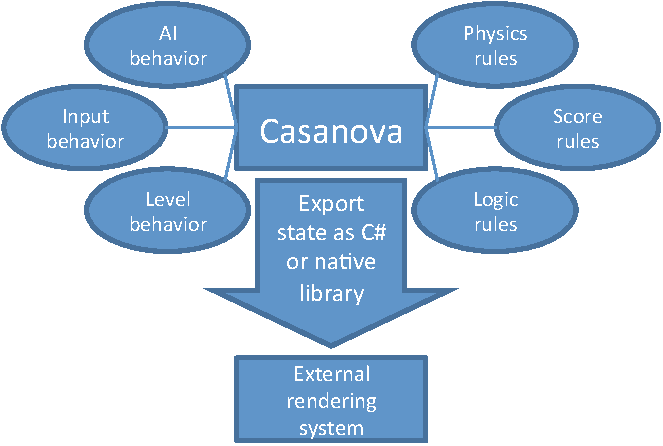
\includegraphics[width=0.5\textwidth]{architecture.pdf}
\caption{Game architecture with Casanova}
\noindent
%\hrulefill
\label{test}
\end{wrapfigure}

Behaviors are used to make it easier to build complex input, articulated level logics or customized AI algorithms into the game. While Casanova does not (yet) integrate any deduction engine or proper AI system, it makes integrating such a system with the game loop and the game state much simpler.

Rules are used to build all the regular logic that the game continuously repeats, for example the fact that when projectiles collide with an asteroid then the asteroid is damaged or other logical relationships between entities. Rules are the main workhorse of a game, and Casanova ensures that all the queries that make up the various rules maintain the integrity of the state and are automatically optimized to yield faster runtime.

The Casanova compiler will then export the game state as a series of type definitions and classes that can be accessed directly (that is without any overhead) from a C\# or C++ rendering library; this way existing rendering code and engines can be integrated with Casanova with little effort.
